%%%%% CPLOP %%%%%
\section{\cploplong{}}

This section details the aspects of \cploplong{} (\cplop{}) relevant to \mstlong{} (\mst{}).
It explains the nature of \pyros{} and the \pyro{}ing process, including what segments of \ecoli{} \dna{} \cplop{} researchers use and how they collect the \isols{} used in the process.
Finally, it describes the steps necessary to properly compare two \ecoli{} \isols{} for strain identification and \mst{} and provides an overview of how \cplop{} stores the \pyro{} data to facilitate it.

%%%%% PYROPRINTS %%%%%
\subsection{\Pyros{}}
\Pyros{} are the core data structure in \cplop{} used to represent \ecoli{} \isols{}.
\index{\pyro{}}
Using an inexpensive \dna{} sequencing technique called pyrosequencing, we can build a fingerprint\footnote{hence, the portmanteau \pyro{}} that allows us to effectively differentiate between \ecoli{} strains.
Building \pyros{} requires careful use of the pyrosequencing process.

Pyrosequencing is a \dna{} sequencing technique appropriate for sequencing short \dna{} fragments (up to around 150-200 base pairs) \cite{ronaghi1998sequencing}.
A machine dispenses a predefined series of nucleotides and carefully measures the light output of the reaction.
The amount of light emitted is directly proportional to the amount of the corresponding nucleotide present in the \dna{}.

The output of the machine is a time series graph depicting the measured light before and after each dispensation.
Previous work in \cite{montana2013algorithms, Shealy:SeniorProject} helped us determine the optimal dispensation order and length and exactly which portions of this graph to use.
Determining the optimal dispensation order and its length are crucial to effective sequencing: too few dispensations may not encode enough information, while too many may degrade the quality of the data.

A \textit{\pyro{}} is a vector representing the peak light values of the pyrosequencing of one of the \itsshort{} regions in the seven loci of the \ecoli{} genome.
\index{\pyro{}}
As explained in \autoref{sec:its}, \Ssixt{} and \Sfive{} offer keen insight into \ecoli{} strains, since random variation can occur in them without affecting the survivability of the \ecoli{} microbes.
We \pyro{} each \itsshort{} separately, building at least two \pyros{} for each \isol{}: one for \Ssixt{} and another for \Sfive{}.

%%%%% ITS %%%%%
\subsection{\ITSlong{}s}\label{sec:its}
Choosing the proper region of \dna{} to fingerprint is crucial to effective strain delineation.
Generally, when fingerprinting \fib{}, researchers avoid using regions that code for functional products and focus instead on non-coding regions of \dna{}, since variations within.
When differentiating between \ecoli{} strains, researchers use the two \itsshort{} regions between three genes: \Gsixt{}, \Gtwen{}, \Gfive{}.

The \Gsixt{}, \Gtwen{}, and \Gfive{} \rrnalong{}s (\rrna{}) are genes that help code for proteins in \ecoli{} bacteria.
\index{\Gsixt{}}
\index{\Gtwen{}}
\index{\Gfive{}}
\index{\rrna{}}
\index{\rrnalong{}}
Any changes to these regions may affect the rate or nature of protein synthesis and thus affect the survivability of the bacteria.
As a result, we consider these regions to remain \textit{conserved} across \ecoli{} strains.
\index{conserved}
Using these segments directly to differentiate between strains would be fruitless, since even wildly different \ecoli{} strains will still have nearly identical copies of these three regions.

Between these three genes are two non-coding, and thus \textit{unconserved}, regions, called \itslong{} (\itsshort{}).
\index{unconserved}
\index{\itslong{}}
\index{\itsshort{}}
Since \itsshort{} do not code for functional products, random variations occur in \itsshort{} regions that do not affect the survivability or reproducibility of the bacteria.
Researchers frequently use \itsshort{} for strain delineation, due to their unconserved nature.
Importantly, any offspring of a microbe inherit the \Ssixt{} and \Sfive{} regions, allowing biologists to use them to differentiate strains \cite{SolimanDVMBNWKG12}.
The two \itsshort{} regions that bridge \Ssixtname{} and \Sfivename{} we respectively refer to as \Ssixt{} and \Sfive{}.
\index{\Ssixtname{}}
\index{\Sfivename{}}
\index{\Ssixt{}}
\index{\Sfive{}}
Amplifying the \itsshort{} regions of \dna{} becomes a straightforward and inexpensive process, due to the highly conserved regions flanking each \itsshort{}.
Primers can reliably attach to the \rrna{} immediately next to each \itsshort{}, because of their conserved nature, allowing for \pcrlong{} (\pcr{}) amplification of the \Ssixt{} and \Sfive{} regions.
\index{\pcrlong{}}
\index{\pcr{}}
\index{\pcr{} amplification}

Applying \pcr{} to an \ecoli{} \isol{} requires awareness of the following principle, crucially affecting how we can interpret a fingerprint:

\begin{principle}[Repeated Loci\index{Repeated Loci Principle}]
The \itsshort{} regions of \ecoli{} and the \rrna{} --- referred to collectively as \textit{loci} --- repeat around the \ecoli{} genome seven times.
\index{loci}
\end{principle}

\begin{figure}
    \centering
    %\begin{tikzpicture}[scale=1.2]
%% Draw three filled circles for points a,x,b, and define 
%% them as TikZ nodes
%\footnotesize
%
%\coordinate (a) at (0,0);
%\coordinate (b) at (1,0);
%\coordinate (c) at (2,0);
%\coordinate (d) at (3,0);
%\coordinate (e) at (4,0);
%\coordinate (f) at (5,0);
%\coordinate (g) at (6,0);
%\coordinate (h) at (7,0);
%
%
%% Label the points
%\draw[line width=1pt]  (a) -- (h);
%\draw[line width=5pt] (b) -- (c);
%\draw[line width=5pt] (d) -- (e);
%\draw[line width=5pt] (f) -- (g);
%
%\node at (1.5,0)[above=5pt] {\Gsixt{}};
%\node at (3.5,0)[above=5pt] {\Gtwen{}};
%\node at (5.5,0)[above=5pt] {\Gfive{}};
%
%\draw[thick, decorate,decoration={brace,amplitude=5pt, mirror}] (c) -- (d)
%node [black,midway,below=5pt] {\Ssixt{}};
%
%\draw[line width=1pt, decorate,decoration={brace,amplitude=5pt, mirror}] (e) -- (f)
%node [black,midway,below=5pt] {\Sfive{}};
%
%\end{tikzpicture}

\newsavebox\greyBox
\begin{lrbox}{\greyBox}
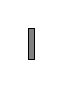
\begin{tikzpicture}[scale=0.04]
\draw[fill=gray] (-1,5)rectangle(1,-5);
\end{tikzpicture}
\end{lrbox}

\newsavebox\blackBox
\begin{lrbox}{\blackBox}

\begin{tikzpicture}[scale=0.04]
\draw[fill=black] (-1,5)rectangle(1,-5);
\end{tikzpicture}
\end{lrbox}

\newsavebox\region
\begin{lrbox}{\region}
\begin{tikzpicture}[scale=1.5]
% Draw three filled circles for points a,x,b, and define 
% them as TikZ nodes
\footnotesize

\coordinate (a) at (0,0);
\coordinate (b) at (1,0);
\coordinate (c) at (2,0);
\coordinate (d) at (3,0);
\coordinate (e) at (4,0);
\coordinate (f) at (5,0);
\coordinate (g) at (6,0);
\coordinate (h) at (7,0);


% Label the points
\draw  (a) -- (b);
\draw[thick, color=cpgreen] (c)--(d);
\draw[thick, color=cpgold] (e)--(f);
\draw  (g) -- (h);
\draw[fill=white] (1,5pt)rectangle(2,-5pt) node[pos=.5]{\Gsixt{}};
\draw[fill=white] (3,5pt)rectangle(4,-5pt) node[pos=.5](gtwen){\Gtwen{}{}};
\draw[fill=white] (5,5pt)rectangle(6,-5pt) node[pos=.5]{\Gfive{}};


\node[below of=gtwen, text width=30, align=center, yshift=8pt] (rna) {rRNA Operon};
\coordinate[below of=rna, yshift=-8pt] (bottom);

\draw[dashed](bottom)--(a);
\draw[dashed](bottom)--(h);

\draw[decorate,decoration={brace,amplitude=5pt}] (c) -- (d)
node [black,midway,above=5pt] {\Ssixt{}};
\draw[decorate,decoration={brace,amplitude=5pt}] (e) -- (f)
node [black,midway,above=5pt] {\Sfive{}};
\end{tikzpicture}
\end{lrbox}

\begin{tikzpicture}[scale=2]
    \draw (0,0) circle (1);
    \node (top) at (90:1) {\usebox\greyBox};
    \node[rotate around={170:(0,0)}] at (80:1) {\usebox\greyBox};
    \node[rotate around={10:(0,0)}] at (100:1) {\usebox\blackBox};
    \node[rotate around={20:(0,0)}] at (110:1) {\usebox\blackBox};
    \node[rotate around={30:(0,0)}] at (120:1) {\usebox\greyBox};
    \node[rotate around={90:(0,0)}] at (180:1) {\usebox\blackBox};
    \node[rotate around={160:(0,0)}] at (250:1) {\usebox\blackBox};
    \node[above of=top, yshift=16pt] {\usebox\region};
\end{tikzpicture}
    \caption{A diagram of a simplified segment of \ecoli{} DNA, outlining the \Ssixt{} and \Sfive{} \itsshort{} regions, which repeat 7 times around the \ecoli{} genome.}
    \label{fig:regionsdiagram}
\end{figure}
\autoref{fig:regionsdiagram} depicts these seven loci and the relative position of the \itsshort{} regions between the \rrna{}.
The primers used to attach to the \rrna{} attach to each of the seven instances, resulting in \pcr{} amplification of all seven copies of \Ssixt{} and \Sfive{}.
What results from \pcr{} is an amplified mixture of these seven unconserved \itsshort{} regions that we can use as a fingerprint for the \isol{}.


The repeating of the \itsshort{} regions makes \pyros{} different from traditional pyrosequencing.
Traditional pyrosequencing allows researchers to figure out the sequence of nucleotides that make up the segment of \dna{}, because they only pyrosequence the \pcr{} amplification of a single segment --- or multiple conserved segments --- at a time.
\Pyro{}ing considers the \pcr{} amplification of more than one unconserved segment of \dna{} at a time, encoding more information with a single \pyro{}.
As a result, \cplop{} researchers cannot use a \pyro{} to figure out the nucleotide sequence of the \pyro{}ed \itsshort{} region.

%%%%% ISOLATES %%%%%
\subsection{Obtaining \& Comparing \ecolilong{} \Isols{}}
\cp{} students collect \ecolilong{} (\ecoli{}) \isols{} from the fecals samples of a variety of different sources and compare them for a multitude of different studies.
Culturing and \ecoli{} extraction occurs in an introductory cell and molecular biology class.
Comparing two \isols{} requires separate consideration of each \itsshort{} region.

The data stored in \cplop{} are obtained as follows.
Biologists collect fecal sample from a host-subject of a known species.
They extract \ecoli{} and culture individual bacterial cells from the bacterial material contained in each sample.
A bacterial \textit{\isol{}} is an individual culture grown from a fecal sample.
\index{\isol{}}
Each \isol{} undergoes \pcr{} procedures that amplify the \dna{} in the two \itsshort{} regions of \dna{}, after which the pyrosequencing of each region produces \pyros{} that are stored in the \cplop{} database.

Sources of \isols{} in \cplop{} are often animal species, but include many \isols{} cultured from environmental sources, like creeks and the ocean.
A large portion of \cplop{} consists of \isols{} derived from Cow and Human sources.
The disproportionate number of Cows in \cplop{} is due to a study investigating the strain demographics and transmission in cattle \cite{dillard2013coli, dillard2015demographics}.
Every year, \cp{} houses cattle from around the state starting in May for testing and vaccination before they leave for auction in September.
\cp{} researchers obtained fecal sample from every cow as they arrived and when they departed, comparing the \isols{} for similarity before and after cohabitation.
\Isols{} derived from Humans make up a large proportion of \cplop{} because \cp{} students investigated \ecoli{} strain characteristics in a variety of studies \cite{neal2013escherichia, montana2012investigating, neal2012demographics}.
Such disproportionate representation of \spec{} in library-based \mst{} is a common problem and \autoref{chap:results} discusses the effect with respect to \cplop{}.

The nature of separately \pyroing{} the \Ssixt{} and \Sfive{} regions of an \isol{} requires adherence to the following principle:

\begin{principle}[Comparing \Isols{}\index{Principle of Comparing \Isols{}}]\label{principle:comparing-isolates}
The only valid comparison between \isols{} using the a comparison metric \pcfunclabel{} is a separate comparison of the \Ssixt{} \pyros{} using \pcfunclabel{} and \Sfive{} \pyros{} using \pcfunclabel{}:
Given two isolates \isola{} and \isolb{}, where 
\isola{} has \pyros{} \isolasixt{} and \isolafive{}
and
\isolb{} has \pyros{} \isolbsixt{} and \isolbfive{},
\pcisolsixt{}
and
\pcisolfive{}
are the only valid comparisons between the two \isols{}.
\end{principle}
\index{comparing \isols{}}
\index{\pearson{}}
\index{\pcfunclabel{}}

\noindent 
In other words, in order to compare two \isols{}, one must consider the \pyros{} of each \itsshort{} region separately, due to the fundamental concept of strains and why we \pyro{} these two regions.
\autoref{fig:isolcompare} depicts the comparison process.
Comparing an \Ssixt{} \pyro{} to an \Sfive{} \pyro{} with \pcfunclabel{} is completely meaningless, since the two \pyros{} represent different segments of \dna{} in the \ecoli{}.

%%%%% PEARSON %%%%%
\subsection{\Pearson{}}
Strain delineation underlies the goals of \cplop{} --- the ability to encode the concept of strains of the \fib{} \ecoli{} and distinguish between different ones is fundamental to library-based \mst{}.
Towards that end, \cplop{} researchers need some way to compare \isols{} using the \pyros{} of their \itsshort{} regions that effectively distinguishes between different strains.
Picking the right comparison function to compare the \pyros{} of two \isols{} is crucial and we found that the \Pearson{} is an effective metric.

%%%%% DEFINITION
Given two \numdims{}-dimensional vectors, $\pcveca{}=\fullvec{\pca{}}{\numdims}$ and $\pcvecb{}=\fullvec{\pcb{}}{\numdims}$, the \pearson{}
%(\pcshort{})
\pcfunclabel{} is:
\begin{equation}\label{eq:pearson}
    \pcfunc{\pca{}}{\pcb{}}
    =
    \pceric{\pca{}}{\pcb{}}
    =
    \frac{\veccov{\pca{}}{\pcb{}}}{\vecstddev{\pca{}}\cdot\vecstddev{\pcb}}
\end{equation}
where $\mu_{\pcveca{}}$, $\mu_{\pcvecb{}}$ are the means of $\pca{}_i$'s and $\pcb{}_i$'s respectively,
$\vecstddev{\pca{}}$, $\vecstddev{\pcb{}}$ are their standard deviations,
and \veccov{\pca{}}{\pcb{}} is the covariance between the two vectors.
\index{\pearson{}}
\index{\pcfunclabel{}}
\index{\pcshort{}}
The \pearson{} encodes a notion of similarity;
as the final portion of \autoref{eq:pearson} shows, \pcshort{} calculates the covariance of the two vectors, normalizing the value by the standard deviation of both.

The \textit{covariance} of two vectors measures the joint variability of the vectors, i.e. how much one vector varies with respect to another.
Given two \numdims{}-dimensional vectors, $\pcveca{}=\fullvec{\pca{}}{\numdims}$ and $\pcvecb{}=\fullvec{\pcb{}}{\numdims}$:
\begin{equation}
    \veccov{\pca{}}{\pcb{}} = \covfull{\pca{}}{\pcb{}}
\end{equation}
\index{covariance}
Positive covariance between two vectors means the two behave similarly, while negative means they behave in the opposite manner. 

The \textit{standard deviation} measures the amount of deviation a set of values has from its average.
Given a \numdims{}-dimensional vector $\pcveca{}=\fullvec{\pca{}}{\numdims}$, its standard deviation is:
\begin{equation}
    \vecstddev{\pca{}} = \stddevfull{\pca{}} 
\end{equation}
\index{standard deviation}
One can also define the standard deviation as the square root of the covariance:
\begin{equation}
    \vecstddev{\pca{}} = \sqrt{\veccov{\pca{}}{\pca{}}}
\end{equation}

Using the \pearson{} as a measure of similarity is straightforward, due to it being a combination of the covariance and the standard deviation.
Since one can define the covariance of a vector with itself in terms of the standard deviation:
\begin{equation}
    \veccov{\pca{}}{\pca{}} = \vecstddev{\pca{}}^2
\end{equation}
it is clear that given two vectors, \pcveca{} and $\pcveca{}\,'$, where $\pcveca{} = \pcvecaa{}$:
\begin{equation}
    \pcfunclabel({\pcveca{}},{\pcvecaa{}})
    = \frac{\cov{\pcveca{}}{\pcvecaa{}}}{\stddev{\pcveca{}}\stddev{\pcvecaa{}}}
    = \frac{\cov{\pcveca{}}{\pcveca{}}}{\stddev{\pcveca{}}\stddev{\pcveca{}}}
    = \frac{\stddev{\pcveca{}}^2}{\stddev{\pcveca{}}^2}
    = 1
\end{equation}
Due to the normalizing effect of the $\sigma{}$'s, it is impossible for $\pcfunclabel{} > 1$.
Conversely, two very dissimilar vectors will have a $\pcfunclabel{} < 1$.
Specifically, \pearson{} measures a linear correlation between vectors, so two vectors with a $\pcfunclabel{} = 0$ means that the two vectors have no linear relationship\footnote{For completeness, if $\pcfunclabel{} \approx -1$, then there is an \textit{inverse correlation} between the two vectors. It is easy to see if 
given $\pcveca{} = \fullvec{\pca{}}{\numdims{}}$
and $\pcvecaa{}=\fullvec{\pca{}'}{\numdims{}} = \fullvec{-\pca{}}{\numdims{}}$,
then $\cov{\pcveca{}}{\pcvecaa{}} = -\veccov{\pca{}}{\pca{}}\Rightarrow\pcfunclabel{(\pcveca{}, \pcvecaa{}) = -\pcfunc{\pca{}}{\pca{}}} = -1$. By similar reasoning, $-1 \leq \pcfunclabel{} \leq 1$
}.
Work done in \cite{Shealy:SeniorProject} determined that multiple \pyros{} of the same \isol{} obtain a $\pcfunclabel{} > 0.995$ and \cplop{} researchers use this value for quality control \cite{kent2014pyroprinting, Black2014121}.

It is from this measure of similarity \pcfunclabel{} that we define a comparison metric between \pyros{}.
The nature of this function works perfectly for what \pyros{} encode.
The values in a \pyro{} represent peak light intensity values from chemical reactions, the intensity of which is proportional to the nucleotide content of the \dna{} \pyro{}ed.
Peak intensity differences and noise from the machine are accounted for by \pearson{}, since it measures how the \pyro{} vector values change with respect to each other and machine variations will be similar between \pyro{}ings.

\begin{figure}
    \centering
    
    \newsavebox\chickenFiveOne
\begin{lrbox}{\chickenFiveOne}
\begin{tikzpicture}[scale=0.8]
\begin{axis}[xticklabels={,,}, yticklabels={,,}, ticks=none, width=3in, height=1in]
\addplot[ybar interval=1, color=cpgreen, fill=cpgreen] 
table [col sep=comma] {data/pyroprints/ck005/4063.csv};
\end{axis}
\end{tikzpicture}
\end{lrbox}

\newsavebox\chickenFiveTwo
\begin{lrbox}{\chickenFiveTwo}
%\resizebox {3in} {1in} {
\begin{tikzpicture}[scale=0.8]
\begin{axis}[xticklabels={,,}, yticklabels={,,}, ticks=none, width=3in, height=1in]
\addplot[ybar interval=1, color=cpgold, fill=cpgold] 
table [col sep=comma] {data/pyroprints/ck005/4039.csv};
\end{axis}
\end{tikzpicture}
\end{lrbox}

\newsavebox\chickenSevenOne
\begin{lrbox}{\chickenSevenOne}
%\resizebox {3in} {1in} {
\begin{tikzpicture}[scale=0.8]
\begin{axis}[xticklabels={,,}, yticklabels={,,}, ticks=none, width=3in, height=1in]
\addplot[ybar interval=1, color=cpgreen, fill=cpgreen] 
table [col sep=comma] {data/pyroprints/ck007/4065.csv};
\end{axis}
\end{tikzpicture}
\end{lrbox}

\newsavebox\chickenSevenTwo
\begin{lrbox}{\chickenSevenTwo}
\begin{tikzpicture}[scale=0.8]
\begin{axis}[xticklabels={,,}, yticklabels={,,}, ticks=none, width=3in, height=1in]
\addplot[ybar interval=1, color=cpgold, fill=cpgold] table [col sep=comma] {data/pyroprints/ck007/4041.csv};
\end{axis}
\end{tikzpicture}
\end{lrbox}
\begin{tikzpicture}[node distance=.35in]
    \node (origin) at (0, 0) {};
    \node (chickenFiveOne) at (-2.25-\isolsep, 2) {
        \usebox\chickenFiveOne
    };
    \node[below of=chickenFiveOne]{\Ssixt{}$_A$};
    \node (chickenFiveTwo) at (-2.25-\isolsep, -2) {
        \usebox\chickenFiveTwo
    };
    \node[below of=chickenFiveTwo]{\Sfive{}$_A$};
    \node (chickenSevenOne) at (2.25+\isolsep, 2)  {
        \usebox\chickenSevenOne
    };
    \node[below of=chickenSevenOne]{\Ssixt{}$_B$};
    \node (chickenSevenTwo) at (2.25+\isolsep, -2) {
        \usebox\chickenSevenTwo
    };
    \node[below of=chickenSevenTwo]{\Sfive{}$_B$};
    
    \node[above of=chickenFiveOne]{\Isol{} $A$};
    \node[above of=chickenSevenOne]{\Isol{} $B$};
    
    %\draw[dashed] (-.5,-2.5)--(-4,-2.5)--(-4,2.5)--(-.5,2.5)--cycle;

    %\draw[dashed]   (.5,-2.5)--(4,-2.5)--(4,2.5)--(.5,2.5)--cycle;
    \draw[dashed] (-5-\isolsep,3.5) rectangle (-1.5,-3.5);
    \draw[dashed] (5+\isolsep,3.5) rectangle (1.5,-3.5);

    \path[<->]
            (chickenFiveOne) 
            edge[bend right] node[below, fill=white] {$\pcfunclabel(\text{\Ssixt{}}_A,\text{\Ssixt{}}_B)$} 
            (chickenSevenOne)

            (chickenFiveTwo) 
            edge[bend right] node[below, fill=white] {$\pcfunclabel(\text{\Sfive{}}_A,\text{\Sfive{}}_B)$} 
            (chickenSevenTwo)
    ;
\end{tikzpicture}
    
    \caption{Comparing \isols{} involves comparing the \pyros{} of each \isol{} using \pcfunclabel{}, the \pearson{}, with the stipulation that one can only compare \pyros{} from the same \itsshort{} in their respective \isol{}. The green bar plots represent a \pyro{} of \Ssixt{}, while gold bar plots represent a \pyro{} of \Sfive{}.}
    \label{fig:isolcompare}
\end{figure}

Defining strains using the \pearson{} requires a similarity threshold, above which we may consider two \isols{} to be part of the same strain.
\index{defining strains}
Two \isols{} are considered to be of the same strain if the \pyros{} of both regions have a $  > \a{}$, where $\a{} = 0.990$ \cite{Shealy:SeniorProject, Black2014121}.
\index{\a{}}
Work done in \cite{Shealy:SeniorProject} determined this \a{} threshold by simulating the \pyro{}ing process with tools from \cite{montana2013algorithms} on known \ecoli{} strains from the \ncbilong{} database.
Simulations performed in \cite{DBLP:conf/bibm/BrandtMSBGK12} further confirmed the usefulness of this \a{} value.

%%%%% DATABASE %%%%%
\subsection{Database}
There are three pieces that comprise \cplop{}: the physical cold storage of fecal samples and \isols{}, the backend data store, and the frontend web interface.
Cold storage allows \cplop{} researchers to perform 
The backend data store holds the \pyros{} and metadata about their \spec{} and collection.
The web interface, shown in \autoref{fig:front-page}, allows researchers to perform queries and test whether \isols{} match.
\begin{figure}
    \centering
    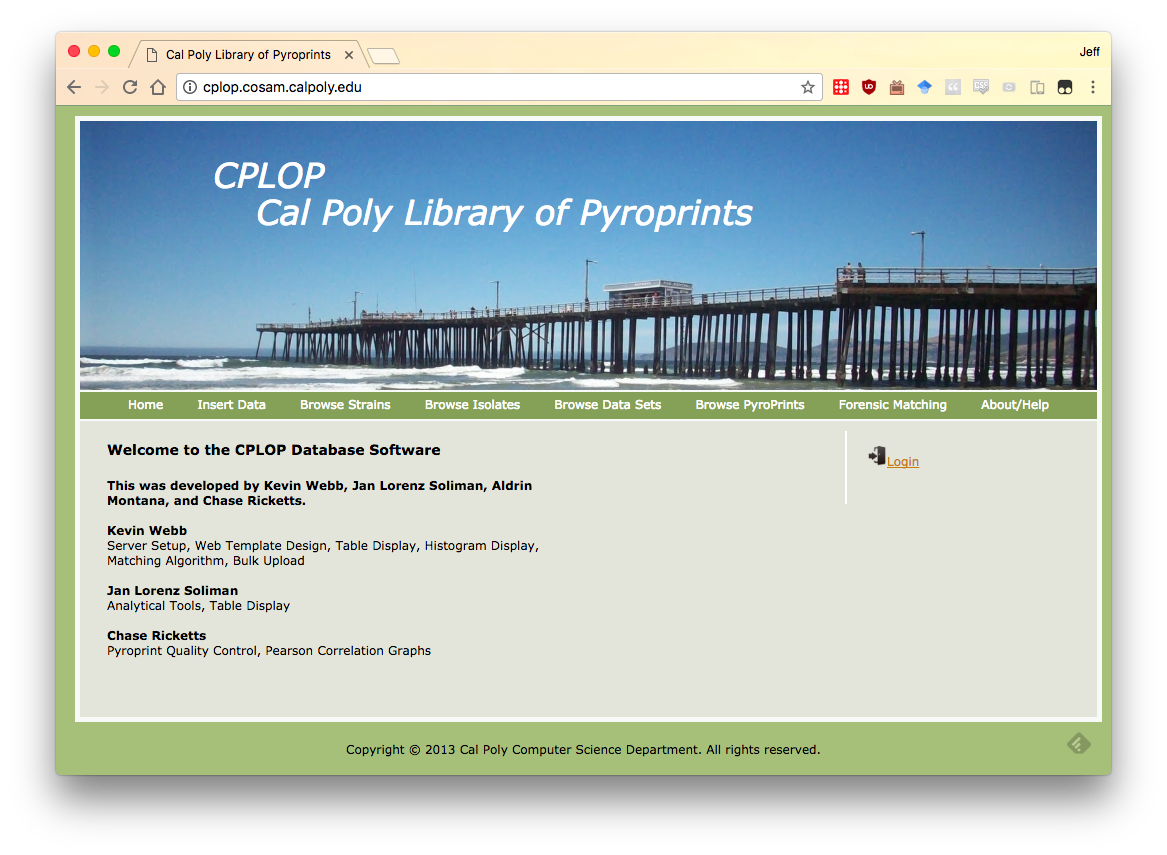
\includegraphics[width=\frontendwidth]{figures/frontend/front-page}
    \caption{Researchers use \cplop{} through a web-accessible frontend.}
    \label{fig:front-page}
\end{figure}

Cold storage holds the collected fecal samples and the \isols{} cultured from them.
It allows \cplop{} researchers to culture additional \isols{} and re-\pyro{} existing \isols{}.
Often, researchers refer to the cold storage as the ``library'' in library-based \mst{}.

The data store for \cplop{} \pyros{} is a \mysql{} database.
It stores metadata for each collected sample, including who collected it and where and when they collected it.
Importantly, the name of the \spec{} and a unique designation for the \host{} marks the sample that the \pyros{} of an \isol{} came from.
For computationally intense 

The web frontend, written in \php{}, allows \cplop{} to access the information in the database from the Internet to: perform queries for \isols{} and \pyros{}, browse \isol{} and \pyro{} datasets, and perform forensic matching. 
The \isols{} in \cplop{} are visible from this interface (see \autoref{fig:browse}) as are the \pyros{}.
\begin{figure}
    \centering
    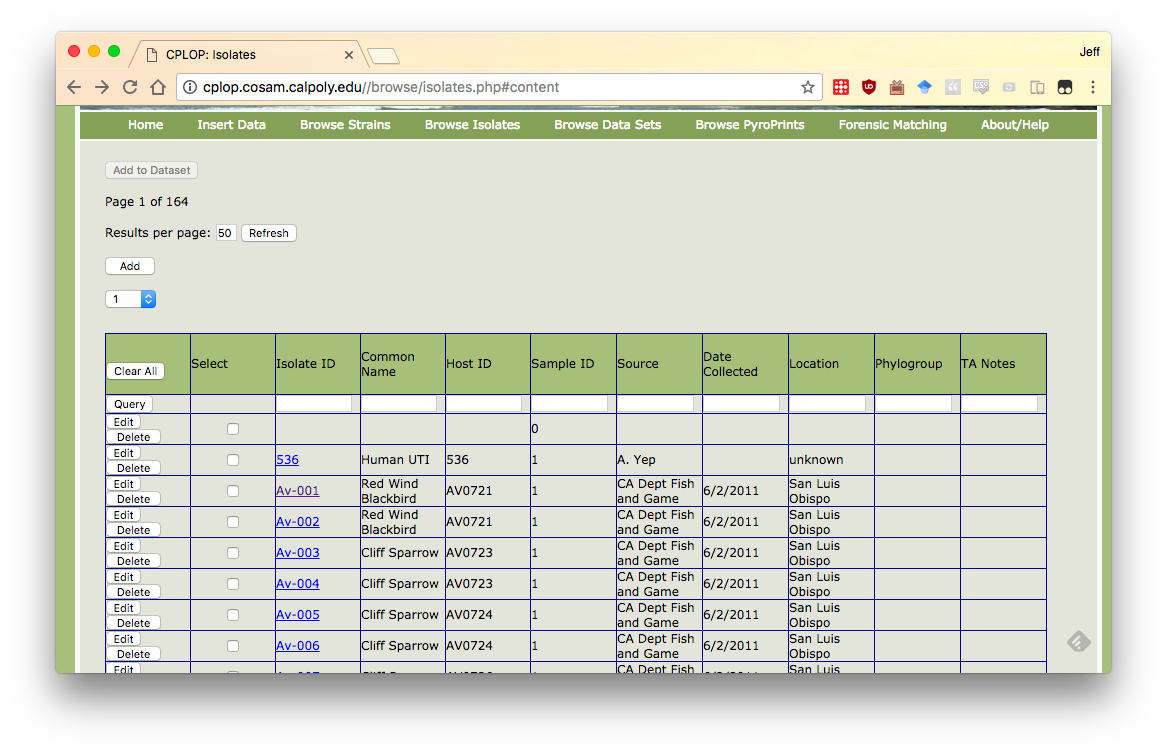
\includegraphics[width=\frontendwidth]{figures/frontend/browse-isolates}
    \caption{\cplop{} allows researchers to explore its \isols{}}
    %\subfloat[Browse \Isols{}]{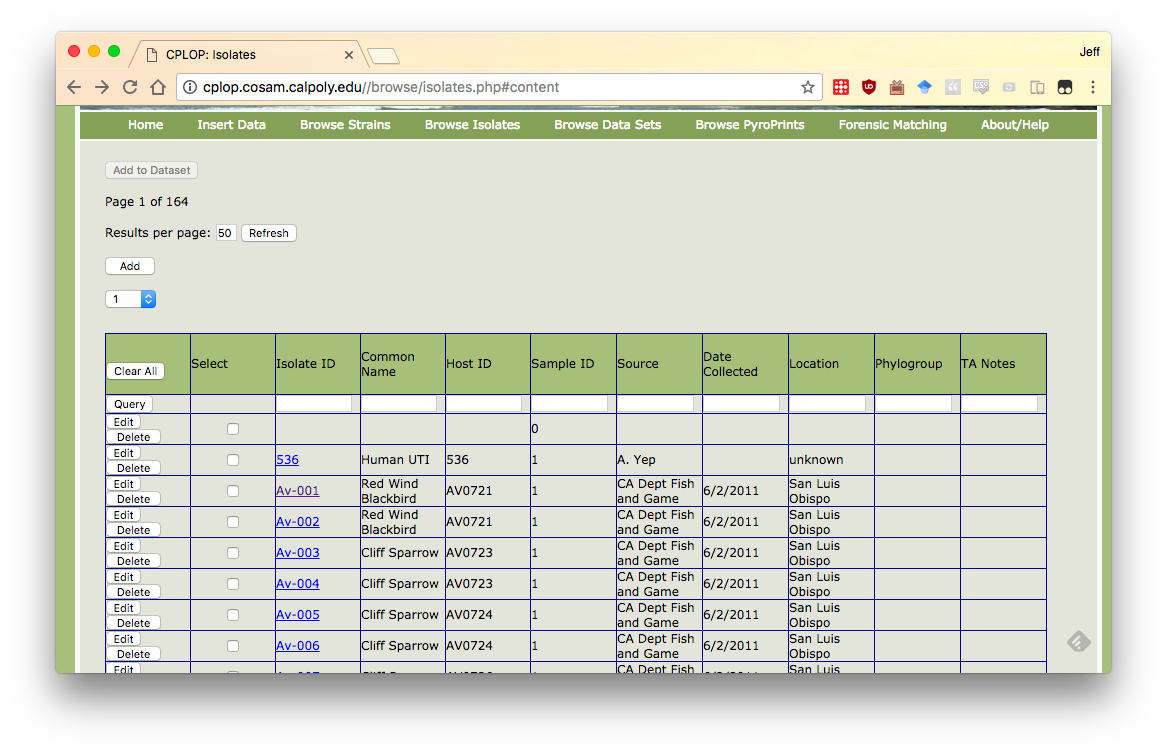
\includegraphics[width=\frontendwidth]{figures/frontend/browse-isolates}\label{fig:browse-isolates}}
    %\\
    %\subfloat[]{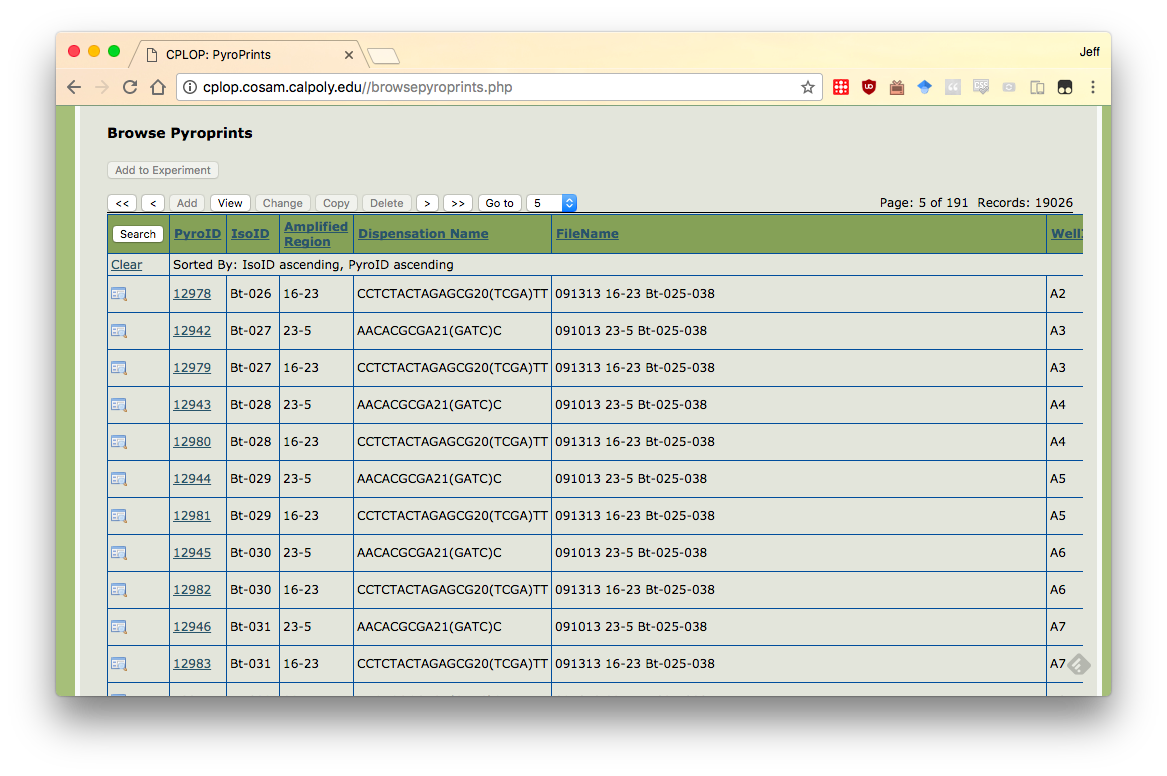
\includegraphics[width=\frontendwidth]{figures/frontend/browse-pyroprints}\label{fig:browse-pyroprints}}
    %\caption{\cplop{} allows researchers to explore its \isols{} \protect\subref{fig:browse-isolates} and \pyros{} \protect\subref{fig:browse-pyroprints}.}
    \label{fig:browse}
\end{figure}
\Isols{} may have multiple \pyros{}, which the \cplop{} frontend allows researchers to browse, which \autoref{fig:browse-isolate-pyroprints} shows.
\begin{figure}
    \centering
    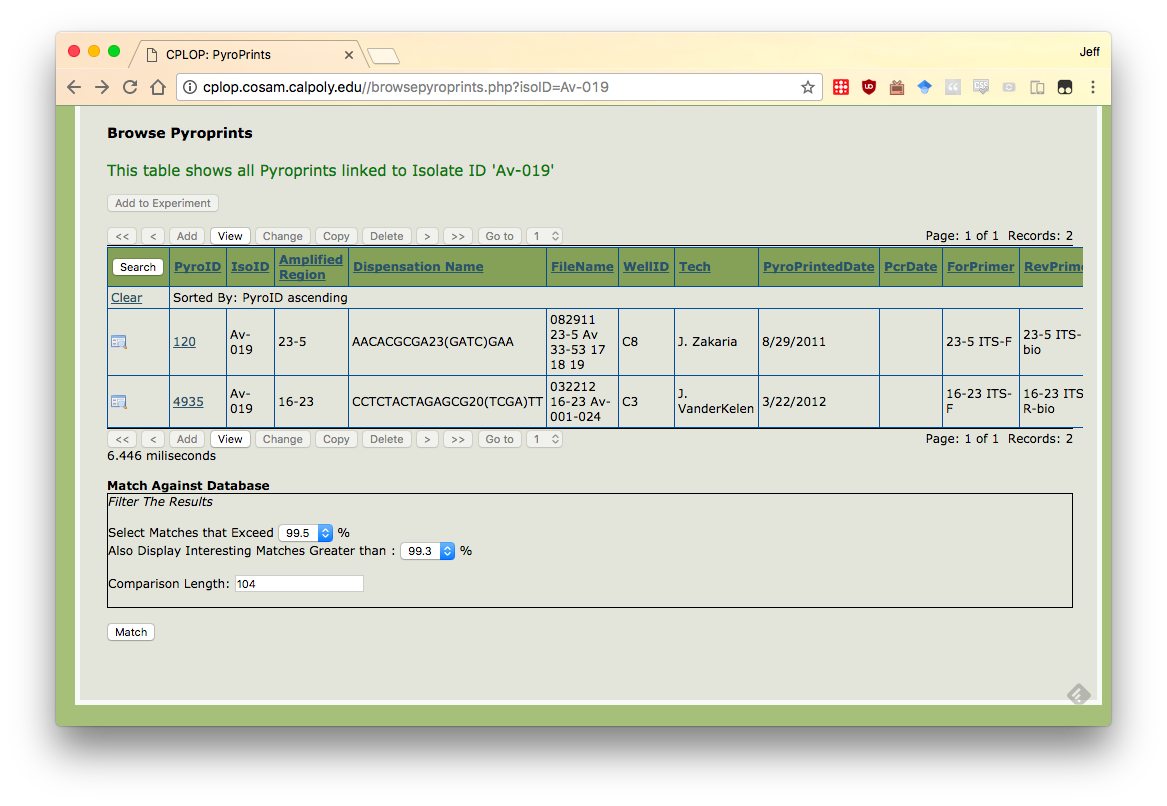
\includegraphics[width=\frontendwidth]{figures/frontend/browse-isolate-pyroprints}
    \caption{The \cplop{} frontend allows researchers to browse the \pyros{} of an \isol{}.}
    \label{fig:browse-isolate-pyroprints}
\end{figure}
Certain \isols{} come from particular collection runs, be they certain studies or classroom examples, and appear collectively as datasets on the website.
\begin{figure}
    \centering
    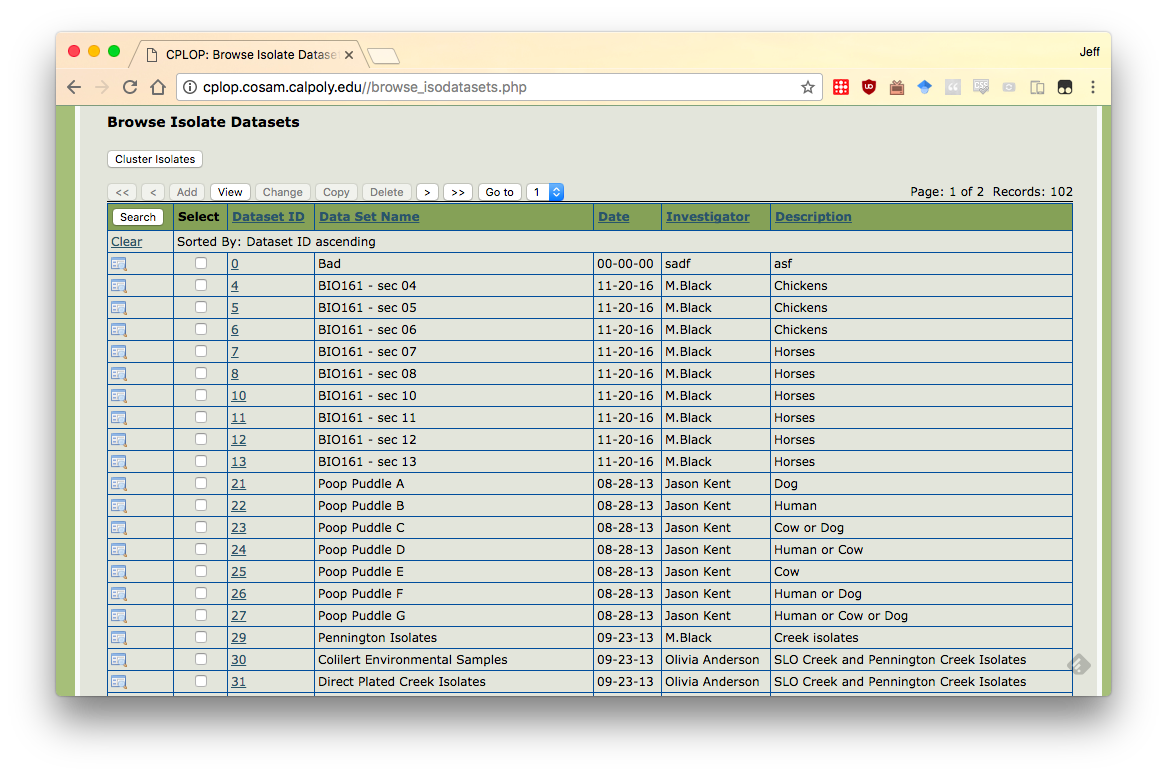
\includegraphics[width=\frontendwidth]{figures/frontend/browse-isolate-datasets}
    \caption{Certain \isols{} may be part of a collection of \isols{}, which \cplop{} has the ability to sort by.}
    \label{fig:browse-isolate-datasets}
\end{figure}
\cplop{} also provides the ability to view the \pyro{} histogram, as \autoref{fig:pyroprint-histogram} shows.
\begin{figure}
    \centering
    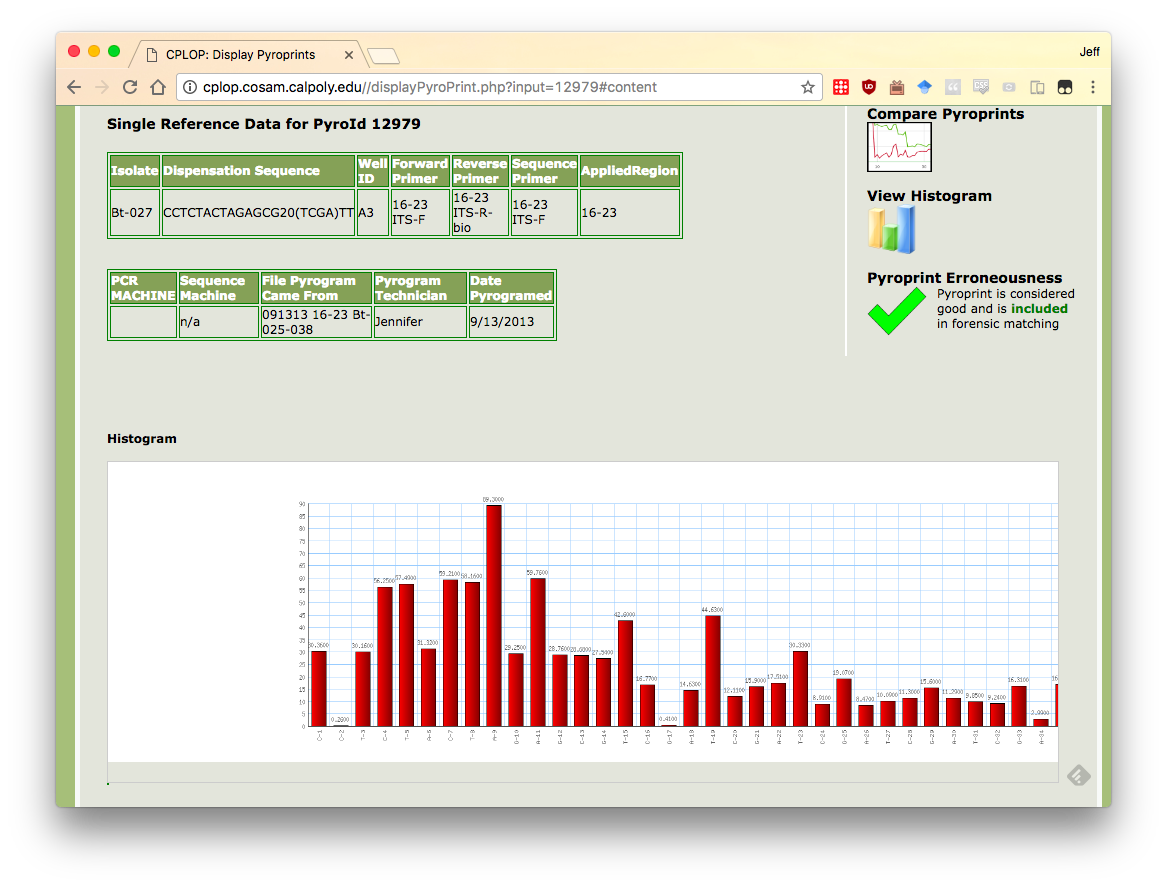
\includegraphics[width=\frontendwidth]{figures/frontend/pyroprint-histogram}
    \caption{Researchers can view the histogram of an individual \pyro{} using \cplop{}.}
    \label{fig:pyroprint-histogram}
\end{figure}
Forensic matching (\autoref{fig:forensic}) is a crucial feature of \cplop{}, allowing researchers to query a dataset against the \cplop{} database to find matching \isols{}.
\begin{figure}
    \centering
    \subfloat[]{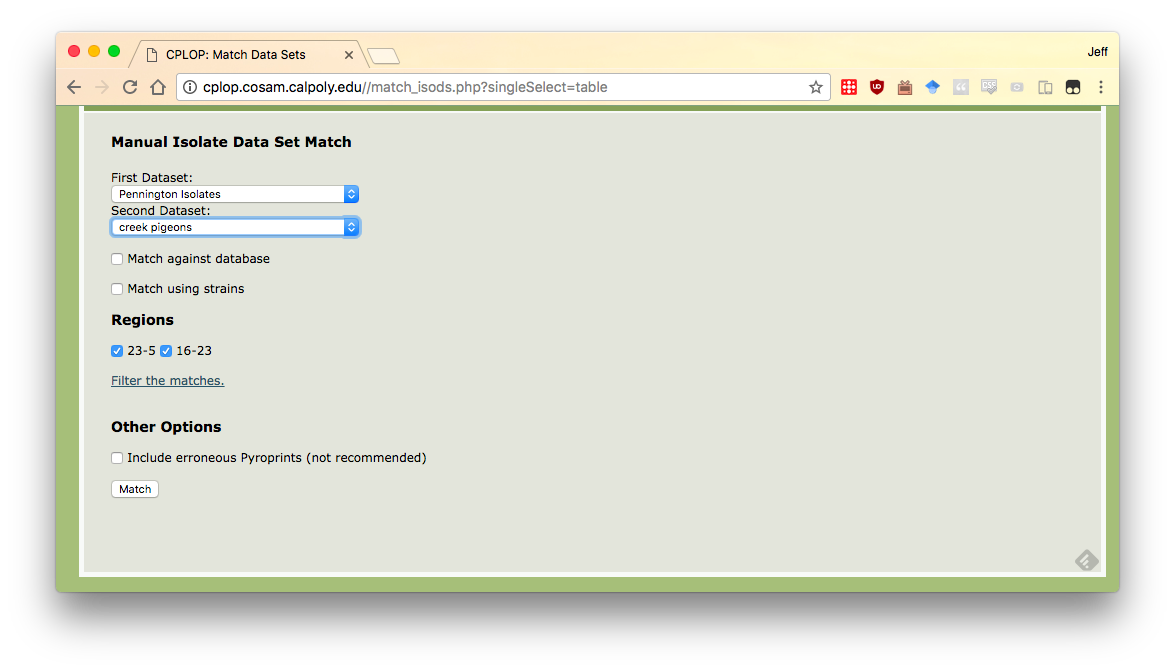
\includegraphics[width=\frontendwidth]{figures/frontend/forensic-choose}\label{forensic-choose}}
    \\
    \subfloat[]{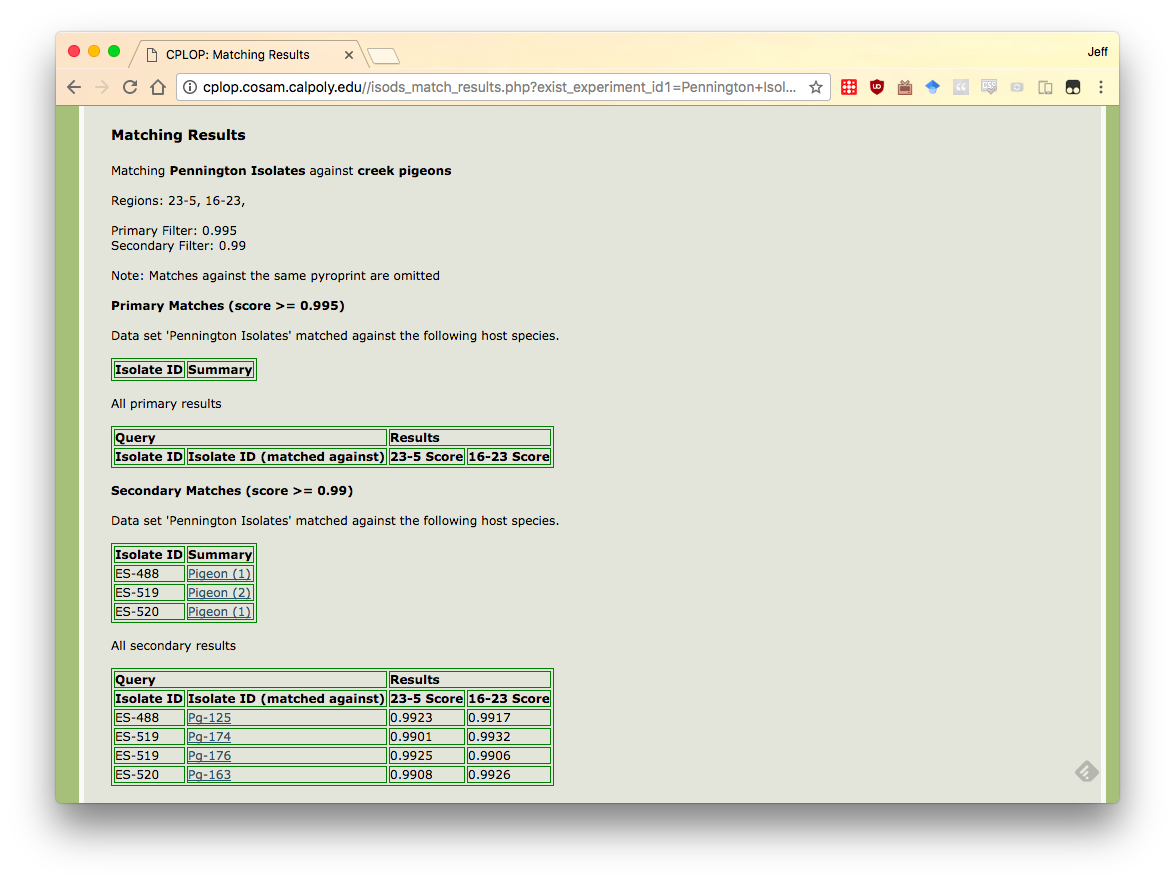
\includegraphics[width=\frontendwidth]{figures/frontend/forensic-result}\label{forensic-result}}
    \caption{Forensic matching is a key feature of \cplop{}, allowing researchers to choose subsets of \cplop{} data \protect\subref{forensic-choose} to find strain-level matches \protect\subref{forensic-result}.}
    \label{fig:forensic}
\end{figure}

\cp{} servers host the \cplop{} website at \url{http://cplop.cosam.calpoly.edu/}.
The servers are limited in computational ability, only containing \gb{4} of \ram{}.
Such limitations make it difficult to implement algorithms like \ohclust{} \cite{montana2013algorithms, montana2013ontological, montana2012investigating}, which require more than \gb{4} of \ram{} for efficient computation, or \cite{adams2016using}, which requires access to a cluster of computers for \mapreduce{} ability.
Future work will assess the feasibility of moving over to more dynamic systems, like \awslong{}.